% !TeX spellcheck = <none>
\documentclass[a4paper, 10pt]{article}

%\usepackage{cmap}
\usepackage[T2A]{fontenc}
\usepackage[utf8]{inputenc}
\usepackage[english, russian]{babel}
\usepackage{graphicx}
\usepackage[top=2cm, bottom=2cm, left=3cm, right=2cm]{geometry}
\graphicspath{./}
\usepackage{biblatex}
\addbibresource{lib.bib}
\linespread{1.5}
{\usefont{T2A}{Tempora-TLF}{m}{n}
\usepackage{amsmath}

\usepackage{ragged2e}
\justifying

\usepackage{listings}
\usepackage{color}


\definecolor{codegreen}{rgb}{0,0.6,0}
\definecolor{codegray}{rgb}{0.5,0.5,0.5}
\definecolor{codepurple}{rgb}{0.58,0,0.82}
\definecolor{backcolour}{rgb}{0.95,0.95,0.92}

\lstdefinestyle{mystyle}{
	backgroundcolor=\color{backcolour},   
	commentstyle=\color{codegreen},
	keywordstyle=\color{magenta},
	numberstyle=\tiny\color{codegray},
	stringstyle=\color{codepurple},
	basicstyle=\ttfamily\footnotesize,
	breakatwhitespace=false,         
	breaklines=false,                 
	captionpos=b,                    
	keepspaces=true,                 
	numbers=left,                    
	numbersep=5pt,                  
	showspaces=false,                
	showstringspaces=false,
	showtabs=false,                  
	tabsize=4
}

\lstset{style=mystyle}

\begin{document}
	
\begin{titlepage}
	\fontsize{12pt}{12pt}\selectfont
	\begin{figure}[t!]
		\centering
		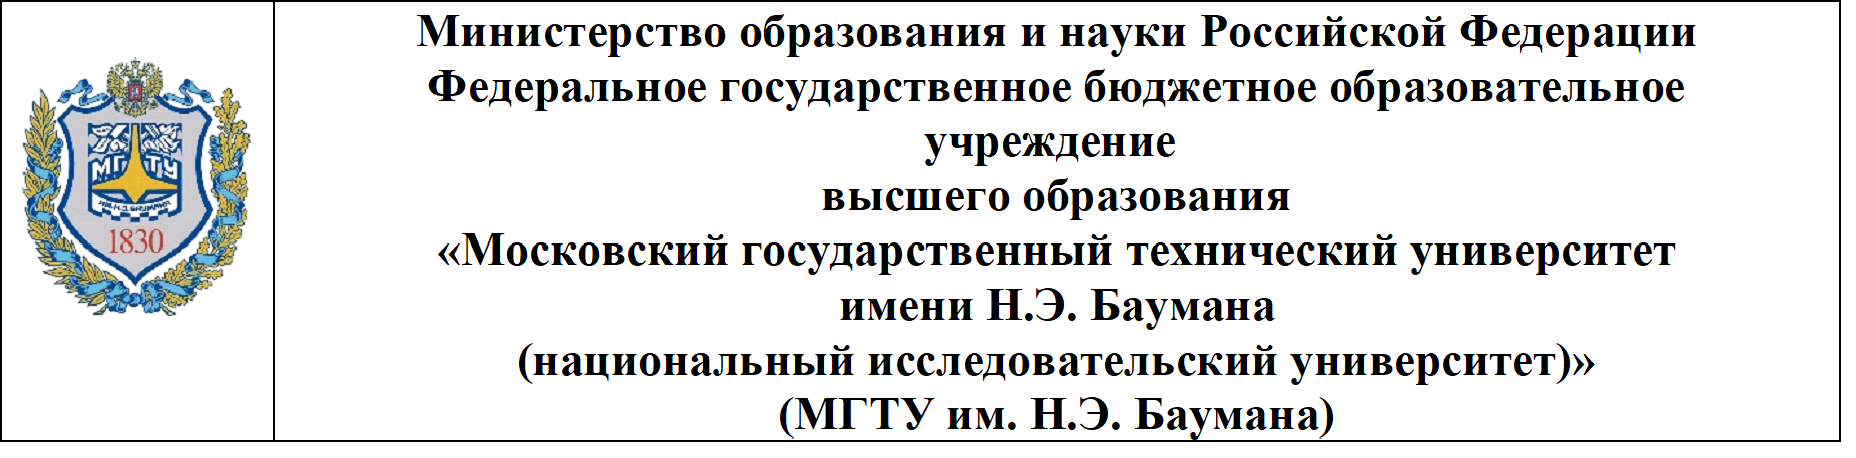
\includegraphics[scale=0.8]{bmstu}
	\end{figure}
	
	\noindent\rule{15cm}{3pt}
	\newline\newline
	\noindent 
	ФАКУЛЬТЕТ 
	\underline{«Информатика и системы управления»} \newline
	
	\noindent КАФЕДРА \underline{«Программное обеспечение ЭВМ и информационные технологии»}\newline\newline\newline\newline\newline
	
	\centering {\Large \textbf{\hspace*{1cm}РАСЧЕТНО-ПОЯСНИТЕЛЬНАЯ ЗАПИСКА}} 
	\newline \\ \centering{\Large \textbf{\textit{\hspace*{20mm}К КУРСОВОЙ РАБОТЕ}}}
	\newline \\ \centering{\Large \textbf{\textit{НА ТЕМУ:}}}
	\vspace{3mm}
	
	\centering{\LARGE \textrm{<<Реализация загружаемого модуля ядра для отслеживания USB-устройств, их идентификации, предоставления или отказа в доступе>>}
		\vspace{10mm}	
		
	\vspace{10mm}}

	\begin{flushleft}
		Студент
		$\underset{\text{  (Группа)}}{\hspace{0.6cm}\underline{\hspace{0.6cm}\text{ИУ7-76Б}\hspace{0.6cm}}}$
		\hspace{30mm}$\underset{\text{(Подипсь, дата)}}{\underline{\hspace{4cm}}}$ 
		\hspace{4mm}$\underset{\text{(И.О.Фамилия)}}{\underline{\text{Ж.Р.Турсунов}}}$ 
	\end{flushleft}

	\begin{flushleft}
		Руководитель курсового проекта
		\hspace{2cm}$\underset{\text{(Подипсь, дата)}}{\underline{\hspace{4cm}}}$ 
		\hspace{4mm}$\underset{\text{(И.О.Фамилия)}}{\underline{\text{Н.Ю.Рязанова}}}$ 
	\end{flushleft} 

	\begin{flushleft}
		Консультант
		\hspace{5.8cm}$\underset{\text{(Подипсь, дата)}}{\underline{\hspace{4cm}}}$ 
		\hspace{4mm}$\underset{\text{(И.О.Фамилия)}}{\underline{\hspace*{3cm}}}$ 
	\end{flushleft}    
	
	\begin{center}
		\vfill
		Москва, \the\year
		~г.
	\end{center}
	\clearpage
	\newpage
	\begin{center}
		\centering{\hspace{10mm} \small \bf Министерство науки и высшего образования Российской Федерации
			Федеральное государственное бюджетное образовательное учреждение
			высшего образования \\ <<Московский государственный технический университет имени Н.Э.Баумана\\(национальный исследовательский университет)>>\\(МГТУ им. Н.Э.Баумана)} 
		\noindent\rule{\textwidth}{2pt}
	\end{center}
	\begin{flushright}
		\normalsize{УТВЕРЖДАЮ \\
			Заведующий кафедрой$\underset{\text{(Индекс)}}{\underline{\text{ИУ7}}}$ 
			\\ \vspace{1mm} $\underset{}{\underline{\hspace{3cm}}}$ \hspace{2mm}$\underset{\text{(И.О.Фамилия)}}{\underline{\text{И.В.Рудаков}}}$
			\\ \vspace{1mm}<<$\underset{}{\underline{\hspace{0.7cm}}}$ >> $\underset{}{\underline{\hspace{3cm}}}$2021 г.} 
	\end{flushright}
	
	\begin{center}
		\large{\bf{ЗАДАНИЕ
				\\ на выполнение курсовой работы}}
	\end{center}
	\begin{flushleft}
		\normalsize{по дисциплене $\underset{}{\underline{\hspace*{1cm} \text{Операционные системы} \hspace*{87mm}}}$
			\\Студент группы \underline{\hspace{1cm} \text{ИУ7-76Б} \hspace{1cm}}
			\\ $\underset{ \text{(Фамилия, имя, отчество)}}{\underline{\hspace*{6cm} \text{Турсунов Жасурбек Рустамович} \hspace*{47mm}}}$
			\\Тема курсовой работы \underline{\text{\hspace{1mm} Реализация загружаемого модуля ядра для отслеживания USB-устройств,}}
			\\ \underline{их идентификации, предоставления или отказа в доступе. \hspace*{65mm}}
			\\ Направленность КР (учебная, исследовательская, практическая, производственная, др.)
			\\ \underline{\hspace{6cm} \text{учебная} \hspace{85mm}}
			\\ Источник тематики (кафедра, предприятие, НИР)\underline{\hspace{2cm} \text{кафедра} \hspace{42mm}}
			\\График выполнения проекта:  25\% к \underline{\hspace*{0.5cm}} нед., 50\% к \underline{\hspace*{0.5cm}} нед., 75\% к \underline{\hspace*{0.5cm}} нед., 100\% к \underline{\hspace*{0.5cm}} нед.}
	\end{flushleft}
	\normalsize {{ \textbf{\textit{Задание}}} \underline{Необходимо реализовать загружаемый модуль ядра для отслеживания изменений в USB-\hspace*{1mm}} \\ \underline{портах и проверки на наличие доступа к секретным файлам. В случае отстутствия допуска - зашиф- } \\ \underline{ровать все запрещенные для копирования файлы.\hspace*{8cm}}}
	\\ \normalsize {{\textbf{\textit{Оформление курсовой работы:}}}}
	\\ Расчетно-пояснительная записка на \underline{20-30} листах формата А4.
	
	\underline{Расчетно-пояснительная записка должна содержать введение, аналитическую часть, конструк-} \\ \underline{торскую часть, технологическую часть, экспериментально-исследовательский раздел, заключение,} \\ \underline{список литературы, приложения. \hspace*{10.5cm}}
	
	\begin{flushleft}
		\small Дата выдачи задания <<\underline{\hspace{1cm}}>> \underline{\hspace{3cm}} 2021 г.
		\newline
		\\ \small \textbf{Руководитель курсового проекта}
		\small \hspace{3cm}$\underset{\text{(Подипсь, дата)}}{\underline{\hspace{4cm}}}$ 
		\small \hspace{4mm}$\underset{\text{(И.О.Фамилия)}}{\underline{\text{Н.Ю.Рязанова}}}$ 
	\end{flushleft}
	\begin{flushleft}
		\small \textbf{Студент}
		\small \hspace{7.2cm}$\underset{\text{(Подипсь, дата)}}{\underline{\hspace{4cm}}}$ 
		\small \hspace{5mm}$\underset{\text{(И.О.Фамилия)}}{\underline{\text{Ж.Р.Турсунов}}}$ 
	\end{flushleft}
	
\end{titlepage}
\setcounter{page}{3}
\tableofcontents
\clearpage
\newpage


\section*{Введение}
\addcontentsline{toc}{section}{Введение}


\hspace*{5mm}Персональные компьютеры, системы управления и сети на их основе быстро входят во все области человеческой деятельности. Среди них можно выделить такие сферы применения, как военная, коммерческая, банковская, научная. Очевидно, широко используя компьютеры для обработки и передачи информации, эти отрасли должны быть надежно защищены от возможности доступа к ней посторонних лиц. Ее утраты или искажения. Согласно данным, более 80\% компаний несут финансовые убытки из-за нарушения целостности и конфиденциальности используемых данных.
\hspace*{5mm} В настоящее время одним из способов защиты персональных данных на компьютере, это доступ к ним по USB-устройству. А именно если вы не хотите, чтобы кто-то извлекал документы, устанавливал вредоносное ПО с вашего компьютера через внешние носители, необходимо отслеживать USB-устройства, их идентифицировать и предоставлять или отказывать в доступе [1]. 
\\ \hspace*{5mm} Linux - это операционная система с монолитным ядром. Для того, чтобы избежать перекомпиляции ядра при добавлении нового функционала, используются загружаемые модули ядра.

\hspace*{5mm}\textbf{Цель данной работы} - реализация загружаемого модуля ядра , для отслеживания USB-устройств, являющихся ключом для секретных файллов.
Для достижения поставленной цели необходимо решить следующие задачи:
\begin{enumerate}
 	\item определение основных понятий;
 	\item разработка алгоритмов;
 	\item реализация загружаемого модуля.
\end{enumerate}
	
\clearpage
\newpage
\section{Аналитическая часть}
	\subsection{Постановка задачи}
	\hspace*{5mm} Требуется разработать программное обеспечение для отслеживания USB-устройств, который обладает следующей функциональностью:
	\begin{enumerate}
		\item список разрешенных устройств;
		\item список путей к секретным файлам;
		\item отслеживание появления новых USB-устройств;
		\begin{enumerate}
			\item если устройство опознано, секретные файлы расшифрованы и доступны;
			\item если устройство не опознано, происходит зашифровка секретных файлов;
		\end{enumerate}
	\end{enumerate}
	\hspace*{5mm} На вход подается USB-устройство с паролем. На выходе получаем зашифрованый или расшифрованный файл.
	
	\subsection{Загружаемый модуль ядра}
	\hspace*{5mm} Ядро Linux динамически изменяемое -- это означает, что вы можете загружать в ядро дополнительную функциональность, выгружать функции из ядра и даже добавлять новые модули, использующие другие модули ядра. Преимущество загружаемых модулей заключается в возможности сократить расход памяти для ядра, загружая только необходимые модули (это может оказаться важным для встроенных систем).
	
	Загружаемый модуль представляет собой специальный объектный файл в формате ELF (Executable and Linkable Format). Для работы с загружаемыми модулями можно использовать стандартные средства работы с объектными файлами (имеют суффикс .ko, от kernel object) [2].
	
	
	В OC Linux существуют специальные команды для работы с загружаемыми модулями ядра:
	\begin{enumerate}
		\item insmod -- Загружает модуль в ядро из конкретного файла, если модуль зависит от других модулей. Только суперпользователь может загрузить модуль в ядро;
		\item lsmod -- Выводит список модулей, загруженных в ядро;
		\item modinfo -- Извлекает информацию из модулей ядра (лицензия, автор, описание);
		\item rmmod -- Команда используется для выгрузки модуля из ядра, в качестве параметра передается имя файла модуля. Только суперпользователь может выгрузить модуль из ядра.
	\end{enumerate}
	
	Загружаемые модули ядра должны содержать два макроса module\_init и module\_exit.
	
	\subsection{Уведомления в ядре Linux}
	\subsubsection{Уведомители}
	\hspace*{5mm} Ядро Linux содержит механизм, называемый <<уведомителями>> (notifiers) или <<цепочками уведомлений>> (notifiers chains), который позволяет различным подсистемам подписываться на асинхронные события от других подсистем. Цепочки уведомлений в настоящее время активно используется в ядре; существуют цепочки для событий hotplug памяти, изменения политики частоты процессора, события USB hotplug, загрузка и выгрузка модулей, перезагрузки системы, изменения сетевых устройств [3].
	
	\subsubsection{Уведомитель изменений на USB портах}
	Существует уведомитель, позволяющий отслеживать изменения на usb портах [4].
	
	\textit{void usb\_register\_notify(struct notifier\_block *nb);}
	
	\textit{void usb\_unregister\_notify(struct notifier\_block *nb);}
	
	\hspace*{-5mm}Существующие события: \textit{USB\_DEVICE\_ADD} -- добавление нового устройства, \textit{USB\_DEVICE\_REMOVE} -- удаление устройства.
	\subsection{Хранение информации о доступных USB-устройствах}
	Для хранения устройств будет использовать двусвязный список ядра Linux, реализованный в файле \#include/linux/list.h [5].
	
	\textit{LIST\_HEAD} -- объявление и инициализация головы списка.
	
	\textit{list\_for\_each\_entry(temp, \&connected\_devices, list\_node)} -- проход по списку.
	
	\textit{list\_for\_each\_entry\_safe(device, temp, \&connected\_devices, list\_node)} -- «защищенный» проход по всем элементам списка, используется для удаления записей списка.
	
	\textit{list\_add\_tail(struct list\_head * new, struct list\_head * head) }-- добавление нового элемента.
	\subsection{Вызов приложения пользовательского пространства из ядра}
	\hspace*{5mm}Usermode-helper API -- это простой API с известным набором опций. Например, чтобы создать процесс из пользовательского пространства, обычно необходимо указать имя исполняемого файла, параметры исполняемого файла и набор переменных среды [6].
	
	\textit{int call\_usermodehelper(const char *path, char **argv, char **envp, int wait)} -- подготовить и запустить приложение пользовательского режима.
	\\ Параметры:
	\begin{enumerate}
		\item \textit{const char * path} -- путь к исполняемому файлц пользовательского режима;
		\item \textit{char ** argv} -- параметры;
		\item \textit{char ** envp} --  переменные среды;
		\item \textit{int wait}  -- дождитесь завершения работы приложения и возврата статуса.
	\end{enumerate}
	
	\subsection{Чтение и запись файлов в пространстве ядра}
	Иногда необходимо читать и записывать файловые данные в ядре Linux [7].
	
	\hspace*{-5mm}В основном это функции: 
	
	\textit{struсt file* filp\_open(const char* filename, int open\_mode, int mode)} -- открытие файла в ядре. filename -- имя файла, который может быть создан или открыт, включает путь до файла; open\_mode -- режим открытия файла O\_CREAT, O\_RDWR, O\_RDONLY, mode -- используется при создании файла, установите разрешения на чтение и запись созданного файла, в противном случае он может быть установлен в 0.
	
	\textit{int filp\_close(struct file*filp, fl\_owner\_t id)} -- закрытие файла.
	
	\textit{ssize\_t vfs\_read(struct file* filp, char \_\_user* buffer, size\_t len, loff\_t* pos)}, \textit{ssize\_t vfs\_write(struct file* filp, const char \_\_user* buffer, size\_t len, loff\_t* pos)} -- чтение и запись файлов в ядре.
	
	Второй параметр этих двух функций имеет перед собой модификатор \_\_user, который требует, чтобы оба указателя буфера указывали на память пространства пользователя. Чтобы эти две функции чтения и записи правильно работали с указателем буфера в пространстве ядра, вам нужно использовать функцию set\_fs(). Ее функция состоит в том, чтобы изменить способ, которым ядро обрабатывает проверку адресов памяти. На самом деле параметр fs этой функции имеет только два значения: USER\_DS и KERNEL\_DS, которые представляют пространство пользователя и пространство ядра соответственно.
	
	\textit{void set\_fs(mm\_segment\_t fs)}
	
	\textit{mm\_segment\_t  get\_fs ()}
	\subsection{Основные используемые структуры}
	\hspace*{5mm} В данной работе приоисходит отслеживание изменений на USB-портах, основными структурами являются usb\_device и usb\_device\_id.
	\subsubsection{usb\_device}
	\hspace*{5mm}Структура usb\_device приведена в листинге \ref{lst:usb_device} -- представление USB-устройста в ядре. Каждое продающееся устройство с USB требует сертификации на соответствие требованиям USB, для чего ему необходимо иметь ID поставщика (vendor ID) и ID изделия (product ID). Эти поля присутствуют в descriptor, используются для идентификации USB устройства.
	\subsubsection{usb\_device\_id}
	\hspace*{5mm}Структура usb\_device\_id приведена в листинге \ref{lst:usb_device_id} -- идентификация USB устройств для отслеживания и подключения.
	
	\hspace*{-5mm}Используемые поля:
	\begin{enumerate}
		\item idVendor -- ID поставщика; 
		\item idProduct -- ID изделия.
	\end{enumerate}

	\subsection{Вывод}
	\hspace*{5mm} В данном разделе была поставлена задача и рассмотрены основные задачи. Также были рассмотрены базовые принципы работы загружаемых модулей ядра, необходимый функционал для работы с USB-устройствами, а также их отслеживание на портах.
\clearpage
\newpage
\section{Конструкторская часть}
	\subsection{Перехват сообщений}
	\hspace*{5mm}Для перехвата сообщений добавление нового USB устройства и удаление USB устройства необходимо в загружаемом модуле ядра разместить уведомитель, принимающий в качества параметра функцию обратного вызова нашей обработки данного события.
	
	Для этого была создана следующая структура представленная в листинге \ref{lst:usb_notify}.
	
	\begin{lstlisting}[language=C, caption = Структура usb\_notify, label=lst:usb_notify]
	static struct notifier_block usb_notify = {
		.notifier_call = notify,
	};
	\end{lstlisting}
	
	В этой структуре содержится указатель на прототип нашей функции обработки:
	
	\hspace*{5mm}\textit{static int notify(struct notifier\_block *self, unsigned long action, void *dev)}
	
	Для создания уведомителя передаем созданную структуру в функцию:
	
	\hspace*{5mm}\textit{usb\_register\_notify(\&usb\_notify);}
	
	Для удаления уведомителя передаем структуру в функцию:
	
	\hspace*{5mm}\textit{usb\_unregister\_notify(\&usb\_notify);}
	\subsection{Хранение информации}
	\hspace*{5mm} Для хранения информации о подключенных USB устройствах создадим структуру, листинг \ref{lst:our_usb_device}.
	
	\begin{lstlisting}[language=C, caption = Структура our\_usb\_device, label =  lst:our_usb_device]
	typedef struct our_usb_device {
		struct usb_device_id dev_id;
		struct list_head list_node;
	} our_usb_device_t;
	\end{lstlisting}
	
	Инициализируем список: \textit{LIST\_HEAD(connected\_devices);}
	
	Для добавления нового подключенного устройства используется функция \ref{lst:add_usb},  для удаления -- \ref{lst:del_usb}.
	\subsection{Алгоритм работы функции-обработчика}
	На рисунке 1 представлен алгоритм работы функции обратного вызова добавления или удаления USB-устройства.
	\clearpage
	\newpage
	\begin{figure}[t!]
		\centering
		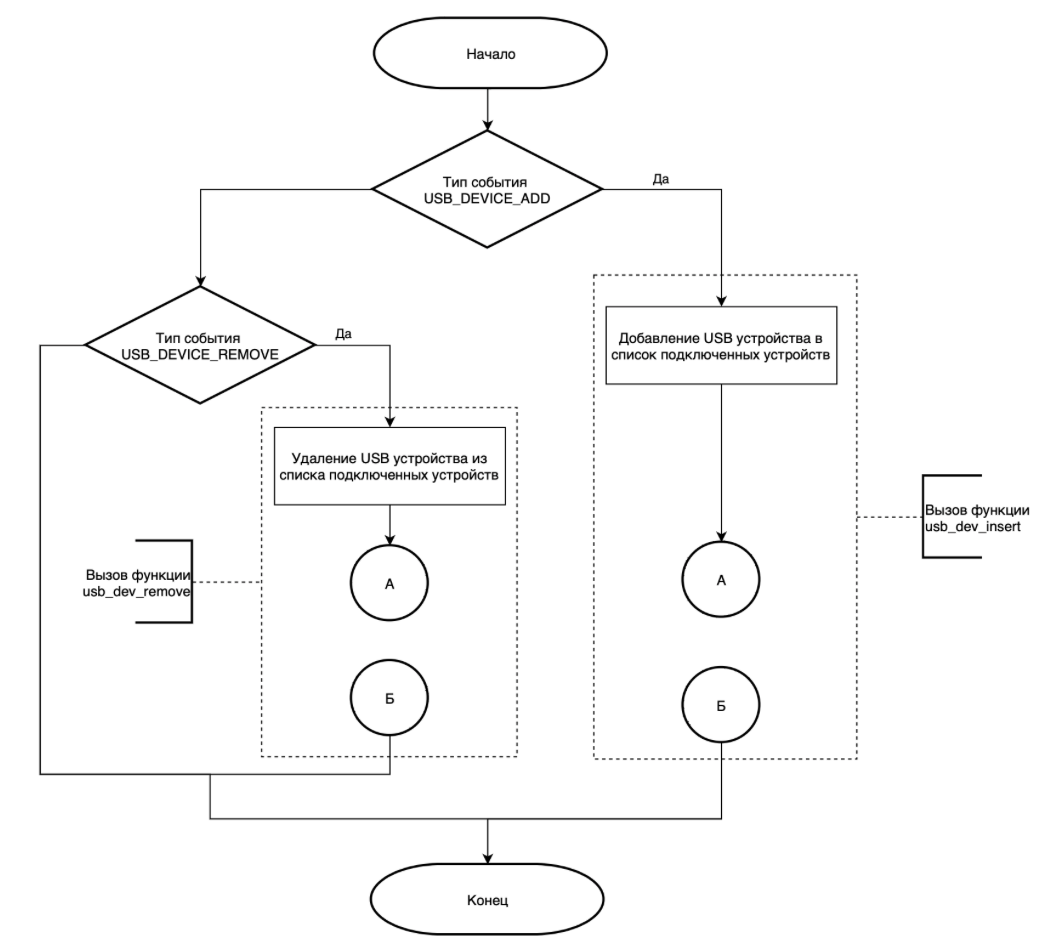
\includegraphics[scale=0.49]{graph1}
		\centering\caption{Алгоритм работы функции-обработчика.}
	\end{figure}
	\clearpage
	\newpage
	\begin{figure}[t!]
		\centering
		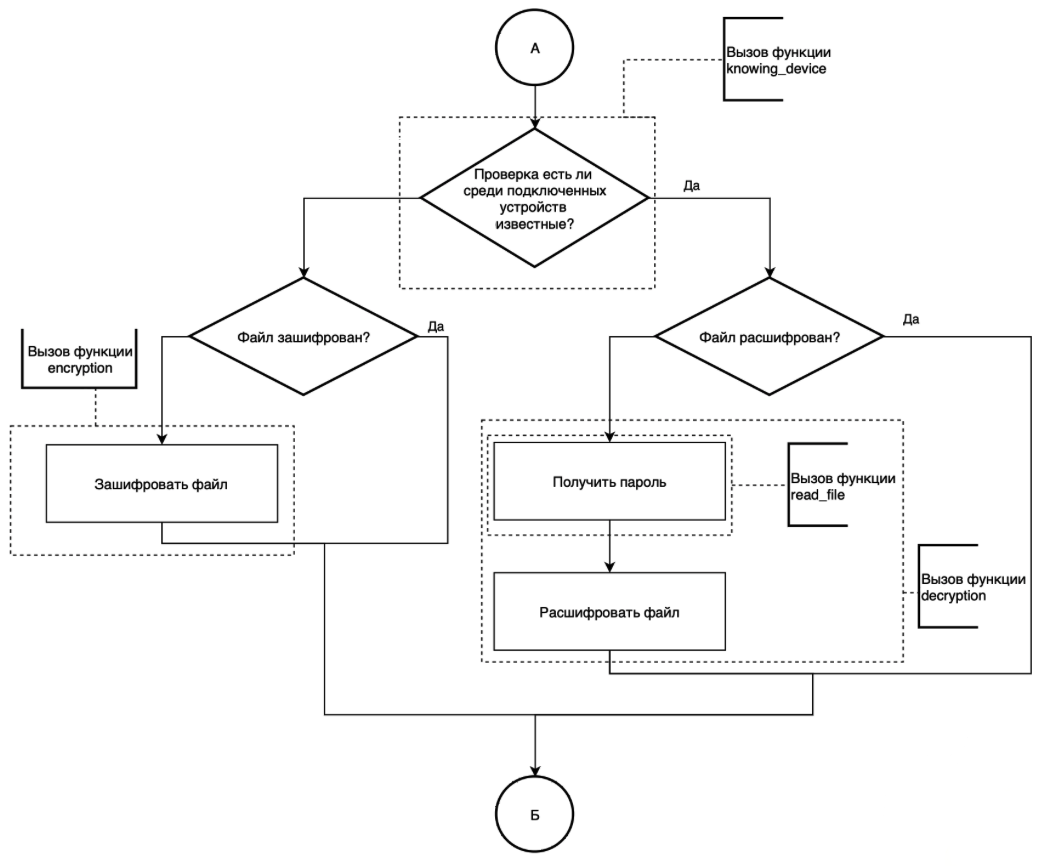
\includegraphics[scale=0.48]{graph2}
		\centering\caption{Алгоритм работы функции-обработчика.}
	\end{figure}
	\subsection{Алгоритм шифрования файла}
	В качестве алгоритма шифрования был выбран самый простой метод:
	\begin{enumerate}
		\item Побайтовое считывание символов из файла;
		\item Применение операции XOR для данных с паролем;
		\item Побайтовая запись символов в файл.
	\end{enumerate}
	\subsection{Вывод}	 
	\hspace*{5mm}Были рассмотрены все необходимые алгоритмы обработки и шифрования, метод хранения информации,  а также был изучен способ перехвата сообщений. Структура программного обеспечения разработа и готова к реализации.
\clearpage
\newpage
\section{Технологическая часть}
	\hspace*{5mm} В данном разделе будут рассмотрены требования к программному обеспечению, средства реализации.
	\subsection{Стек технологий}
	\hspace*{5mm}Для реализации был выбран язык программирования C. Компилятор -- gcc. Для сборки был написан Makefile, позволяющий запускать сборку, одной командой -- листинг \ref{lst:makefile}.  
	\subsection{Хранение данных}
	\hspace*{5mm}Параметры USB устройств, идентификатор поставщика и изделия, а также список секретных файлов и приложений хранятся в конфигурационном файле. Пример конфигурационного файла USB устройств представлен в листинге \ref{lst:config_usb}. Конфигурационный файл секретных файлов и приложений -- листинг \ref{lst:config_file}.
	
	\hspace*{5mm}Пароль для доступа к зашифрованным данным хранится на разрешенном USB устройстве в файле \textit{password.txt}.
	\subsection{Загружаемый модуль}
	Реализация загрузки и удаления представлена в листинге \ref{lst:module}.
	После компиляции загружаемого модуля объектный файл может быть загружен в ядро с помощью команды \textit{insmod} с правами суперпользователя, для выгрузки используется команда \textit{rmmod}.
	\subsection{Функиция-обработчик}
	\hspace*{5mm}В листинге \ref{lst:notify} представлена реализация функции обратного вызова добавления или удаления USB устройства \textit{static int notify(struct notifier\_block *self, unsigned long action, void *dev)}. 
	
	С последующим вызовом, в зависимости от события \textit{static void usb\_dev\_remove(struct usb\_device *dev)}, \textit{static void usb\_dev\_insert(struct usb\_device *dev)}.
	\subsection{Идентификация устройства}
	\hspace*{5mm}Чтобы узнать можно ли расшифровать файл, необходимо узнать принадлежит ли устройство списку разрешенных устройств. Каждое устройство имеет уникальную пару идентификатор поставщика и идентификатор изделия, по ней и будет происходит поиск. Также в известных устройствах хранится файл с паролем для расшифровки секретных данных.
	
	Реализация данной проверки представлена в листинге \ref{lst:check}.
	
	Считывание пароля представлено в листинге \ref{lst:password}.
	
	После проверки принадлежности, при необходимости вызываются функции шифровки и расшифровки файлов, которые вызывают исполняемый файл пользовательского пространства.
	
	Реализация этих функций представлена в листинге \ref{lst:user_call}.
	
	\subsection{Вывод}
	\hspace*{5mm}Реализовано спроектированное программное обеспечение.
	
\clearpage
\newpage
\section{Исследовательская часть }
	\hspace*{5mm} В данном разделе будет проведен эксперимент. Также будут показаны примеры работы программы.
	\subsection{Системные характеристики}
	Характеристики компьютера на котором проводился эксперимент:
	\begin{enumerate}
		\item операционная система - Linux Ubuntu 18.04;
		\item процессор - Intel(R) Core(TM) i7-10510U CPU @1.80GHz 2.30GHz;
		\item объем оперативной памяти - 16 ГБ;
		\item количество ядер - 4;
		\item количество логических процессов - 8;
	\end{enumerate}
	\subsection{Постановка эксперимента}
	В рамках данного проекта были проведены эксперименты, описанные ниже:
	\begin{enumerate}
		\item проверка защищенности секретных файлов при подключение опознанного устройства;
		\item проверка защищенности секретных файлов при подключение неопознанного устройства;
		\item Корректная обработка в случае, если подключено разрешенное и неразрешенное устройства одновременно.
	\end{enumerate}
	\subsection{Пример работы}
	
	\subsection{Вывод}
	Все поставленные эксперименты прошли проверку. Разработанное программное обеспечение отвечает требованиям.
	\clearpage
\section*{Заключение}
	\addcontentsline{toc}{section}{Заключение}
	В результате проделанной работы выполнены следующие задачи.
	\begin{enumerate}
		\item[1. ] Определены основные понятия, такие как загружаемый модуль ядра, уведомления и уведомители. Рассмотрены структуры usb\_device, usb\_device\_id. 
		\item[2. ] Разработаны алгоритмы работы функции-обработчика и шифрования файлов. 
		\item[3. ] Реализован загружаемого модуля. 
	\end{enumerate}
	
	Достигнута цель проекта -- реализация загружаемого модуля ядра для отслеживания USB-устройств, являющихся ключом для доступа к приложению. 
\clearpage
\newpage

\section*{Список литературы}
\addcontentsline{toc}{section}{Список литературы}
[1] \hspace{2mm} Утечки данных 2019: статистика // https://vc.ru/services/103616-utechki-dannyh-2019-statistika-tendencii-kiberbezopasnosti-i-mery-po-snizheniyu-riskov-vzloma (дата обращения: 14.10.2021).\vspace{3mm}
\newline [2]\hspace{2mm} Анатомия загружаемых модулей ядра Linux // https://www.ibm.com/developerworks/ru/library/l-lkm/index.html" (дата обращения: 15.10.2021).\vspace{3mm}
\newline [3]\hspace{2mm} Notification Chains in Linux Kernel// https://0xax.gitbooks.io/linux-insides/content/Concepts/linux-cpu-4.html (дата обращения: 25.10.2021)\vspace{3mm} 
\newline [4]\hspace{2mm} include/linux/usb.h// https://elixir.bootlin.com/linux/latest/source/include/linux/usb.hL2020(дата обращения: 03.11.2021).\vspace{3mm}
\newline [5]\hspace{2mm} Doubly Linked Lists // https://www.kernel.org/doc/html/v4.14/core-api/kernel-api.html (дата обращения: 03.11.2021).\vspace{3mm}
\newline [6]\hspace{2mm} Invoking user-space applications from the kernel // https://developer.ibm.com/technologies/linux/articles/l-user-space-apps/ (дата обращения: 04.11.2021).\vspace{3mm}
\newline [7]\hspace{2mm} Reading and writing of files in Linux kernel driver // https://www.programmersought.com/article/83015124510/ (дата обращения: 04.11.2021).\vspace{3mm}

\clearpage
\newpage


\section*{Листинги}
\addcontentsline{toc}{section}{Листинги}

\begin{lstlisting}[language=C, caption = Структура usb\_device, label =  lst:usb_device]
struct usb_device {
	int		devnum;
	char		devpath[16];
	u32		route;
	enum usb_device_state	state;
	enum usb_device_speed	speed;
	unsigned int		rx_lanes;
	unsigned int		tx_lanes;
	
	struct usb_tt	*tt;
	int		ttport;
	
	unsigned int toggle[2];
	
	struct usb_device *parent;
	struct usb_bus *bus;
	struct usb_host_endpoint ep0;
	
	struct device dev;
	
	struct usb_device_descriptor descriptor;
	struct usb_host_bos *bos;
	struct usb_host_config *config;
	
	struct usb_host_config *actconfig;
	struct usb_host_endpoint *ep_in[16];
	struct usb_host_endpoint *ep_out[16];
	
	char **rawdescriptors;
	
	unsigned short bus_mA;
	u8 portnum;
	u8 level;
	u8 devaddr;
	
	unsigned can_submit:1;
	unsigned persist_enabled:1;
	unsigned have_langid:1;
	unsigned authorized:1;
	unsigned authenticated:1;
	unsigned wusb:1;
	unsigned lpm_capable:1;
	unsigned usb2_hw_lpm_capable:1;
	unsigned usb2_hw_lpm_besl_capable:1;
	unsigned usb2_hw_lpm_enabled:1;
	unsigned usb2_hw_lpm_allowed:1;
	unsigned usb3_lpm_u1_enabled:1;
	unsigned usb3_lpm_u2_enabled:1;
	int string_langid;
	
	/* static strings from the device */
	char *product;
	char *manufacturer;
	char *serial;
	
	struct list_head filelist;
	
	int maxchild;
	
	u32 quirks;
	atomic_t urbnum;
	
	unsigned long active_duration;
	
#ifdef CONFIG_PM
	unsigned long connect_time;
	
	unsigned do_remote_wakeup:1;
	unsigned reset_resume:1;
	unsigned port_is_suspended:1;
#endif
	struct wusb_dev *wusb_dev;
	int slot_id;
	enum usb_device_removable removable;
	struct usb2_lpm_parameters l1_params;
	struct usb3_lpm_parameters u1_params;
	struct usb3_lpm_parameters u2_params;
	unsigned lpm_disable_count;
	
	u16 hub_delay;
	unsigned use_generic_driver:1;
};
\end{lstlisting}

\begin{lstlisting}[language=C, caption = Структура usb\_device\_id, label =  lst:usb_device_id]
struct usb_device_id {
		/* which fields to match against? */
		__u16		match_flags;
		
		/* Used for product specific matches; range is inclusive */
		__u16		idVendor;
		__u16		idProduct;
		__u16		bcdDevice_lo;
		__u16		bcdDevice_hi;
		
		/* Used for device class matches */
		__u8		bDeviceClass;
		__u8		bDeviceSubClass;
		__u8		bDeviceProtocol;
		
		/* Used for interface class matches */
		__u8		bInterfaceClass;
		__u8		bInterfaceSubClass;
		__u8		bInterfaceProtocol;
		
		/* Used for vendor-specific interface matches */
		__u8		bInterfaceNumber;
		
		/* not matched against */
		kernel_ulong_t	driver_info
					__attribute__((aligned(sizeof(kernel_ulong_t))));
	};
\end{lstlisting}

\begin{lstlisting}[language=C, caption = Добавление usb устройства, label =  lst:add_usb]
static void add_our_usb_device(struct usb_device *dev)
{
	our_usb_device_t* new_usb_device = (our_usb_device_t *)kmalloc
							(sizeof(our_usb_device_t), GFP_KERNEL);
	struct usb_device_id new_id = { USB_DEVICE(dev->descriptor.idVendor, 
												dev->descriptor.idProduct) };
	new_usb_device->dev_id = new_id;
	list_add_tail(&new_usb_device->list_node, &connected_devices);
}
\end{lstlisting}

\begin{lstlisting}[language=C, caption = Удаление usb устройства, label =  lst:del_usb]
static void delete_our_usb_device(struct usb_device *dev)
{
	our_usb_device_t *device, *temp;
	list_for_each_entry_safe(device, temp, &connected_devices, list_node) 
	{
		if (device_match_device_id(dev, &device->dev_id))
		{
			list_del(&device->list_node);
			kfree(device);
		}
	}
}
\end{lstlisting}

\begin{lstlisting}[language=C, caption = Makefile, label =  lst:makefile]
ifneq ($(KERNELRELEASE),)
	obj-m := md.o
else
	CURRENT = $(shell uname -r)
	KDIR = /lib/modules/$(CURRENT)/build
	PWD = $(shell pwd)
	
default:
	$(MAKE) -C $(KDIR) M=$(PWD) modules
	
clean:
	rm -rf .tmp_versions
	rm *.ko
	rm *.o
	rm *.mod.c
	rm *.symvers
	rm *.order
	
endif
\end{lstlisting}

\begin{lstlisting}[language=C,caption = Конфигурационный файл USB устройств, label =  lst:config_usb]
struct known_usb_device { 
	struct usb_device_id dev_id;    
	char *name;
};

// List of all USB devices you know
static const struct known_usb_device known_devices[] = {    
	{ .dev_id = { USB_DEVICE(0x0951, 0x1666) }, 
					.name = "Kingston Technology DataTraveler G4" },
};
\end{lstlisting}

\begin{lstlisting}[language=C,caption = Конфигурационный файл секретных файлов и приложений, label =  lst:config_file]  
static char *secret_apps[] = {    
	"/home/jasur/projects/courseWork-OS/code/file.txt",
	NULL,
};
\end{lstlisting}

\begin{lstlisting}[language=C,caption = Загрузка и удаление модуля ядра, label =  lst:module]
static int __init my_module_init(void)
{
	usb_register_notify(&usb_notify);
	call_encryption();
	printk(KERN_INFO "USB MODULE: loaded.\n");
	return 0;
}

static void __exit my_module_exit(void)
{
	usb_unregister_notify(&usb_notify);    
	printk(KERN_INFO "USB MODULE: unloaded.\n");
}

module_init(my_module_init);
module_exit(my_module_exit);
\end{lstlisting}


\begin{lstlisting}[language=C,caption = Функция-обработчик, label =  lst:notify]
// If usb device inserted.
static void usb_dev_insert(struct usb_device *dev)
{   
	add_our_usb_device(dev);
	char *name = knowing_device();
	
	if (name)
	{
		if (state_encrypt)
			call_decryption(name);
		state_encrypt = false;
		printk(KERN_INFO "USB MODULE: New device we can encrypt.\n");
	}
	else
	{
		if (!state_encrypt)
			call_encryption();
		state_encrypt = true;
		printk(KERN_INFO "USB MODULE: New device, we can't encrypt.\n");
	}
}

// If usb device removed.
static void usb_dev_remove(struct usb_device *dev)
{
	delete_our_usb_device(dev);
	char *name = knowing_device();
	
	if (name)
	{
		if (state_encrypt)
			call_decryption(name);
		state_encrypt = false; 
		printk(KERN_INFO "USB MODULE: Delete device, we can encrypt.\n");
	}
	else
	{
		if (!state_encrypt)
			call_encryption();
		state_encrypt = true;
		printk(KERN_INFO "USB MODULE: Delete device, we can't encrypt.\n");
	}
}

// New notify.
static int notify(struct notifier_block *self, unsigned long action, void *dev)
{
	// Events, which our notifier react.
	switch (action) 
	{
		case USB_DEVICE_ADD:
			usb_dev_insert(dev);
			break;
		case USB_DEVICE_REMOVE:
			usb_dev_remove(dev);
			break;
		default:
			break;
	}
	return 0;
}
\end{lstlisting}

\begin{lstlisting}[language=C,caption = Функции для проверки разрешенных устройств, label =  lst:check]
// Match device id with device id.
static bool device_id_match_device_id(struct usb_device_id *new_dev_id, 
			const struct usb_device_id *dev_id)
{
	// Check idVendor and idProduct, which are used.
	if (dev_id->idVendor != new_dev_id->idVendor)
		return false;
	if (dev_id->idProduct != new_dev_id->idProduct)
		return false;
	return true;
}

// Check our list of devices, if we know device.
static char *usb_device_id_is_known(struct usb_device_id *dev)
{
	unsigned long known_devices_len = sizeof(known_devices) / sizeof(known_devices[0]);
	int i = 0;
	for (i = 0; i < known_devices_len; i++)
	{
		if (device_id_match_device_id(dev, &known_devices[i].dev_id))
		{
			int size = sizeof(known_devices[i].name);
			char *name = (char *)kmalloc(size + 1, GFP_KERNEL);
			int j = 0;
			for (j = 0; j < size; j++)
				name[j] = known_devices[i].name[j];
			name[size + 1] = '\0';
			
			return name;
		}
	}
	return NULL;
}

static char *knowing_device(void)
{
	our_usb_device_t *temp;
	int count = 0;
	char *name;
	
	list_for_each_entry(temp, &connected_devices, list_node) {
		name = usb_device_id_is_known(&temp->dev_id);
		if (!name)
			return NULL;
		count++;
	}
	if (0 == count)
		return NULL;
	return name;
}
\end{lstlisting}


\begin{lstlisting}[language=C,caption = Считывание пароля из файла USB устройства, label =  lst:password]
static char *read_file(char *filename)
{
	struct kstat *stat;
	struct file *fp;
	mm_segment_t fs;
	loff_t pos = 0;
	char *buf;
	int size;
	
	fp = filp_open(filename, O_RDWR, 0644);
	if (IS_ERR(fp))
	{
		return NULL;
	}
	
	fs = get_fs();
	set_fs(KERNEL_DS);
	
	stat = (struct kstat *)kmalloc(sizeof(struct kstat), GFP_KERNEL);
	if (!stat)
	{
		return NULL;
	}
	
	vfs_stat(filename, stat);
	size = stat->size;
	
	buf = kmalloc(size, GFP_KERNEL);
	if (!buf) 
	{
		kfree(stat);
		return NULL;
	}
	
	kernel_read(fp, buf, size, &pos);
	
	filp_close(fp, NULL);
	set_fs(fs);
	kfree(stat);
	buf[size]='\0';
	return buf;
}
\end{lstlisting}

\begin{lstlisting}[language=C,caption = Функции вызывающие исполняемый файл пользовательского пространства, label =  lst:user_call]
static int call_decryption(char *name_device) {
	printk(KERN_INFO "USB MODULE: Call_decrypt\n");
	
	char path[80];
	strcpy(path, USB_FOLDER);
	strcat(path, name_device);
	strcat(path, "/");
	strcat(path, PASSWORD_FILE);
	char *data = read_file(path);
	
	char *argv[] = {
		"/home/jasur/projects/courseWork-OS/code/crypto",
		data,
		NULL };
	
	static char *envp[] = {
		"HOME=/",
		"TERM=linux",
		"PATH=/sbin:/bin:/usr/sbin:/usr/bin", 
		NULL };
	
	if (call_usermodehelper(argv[0], argv, envp, UMH_WAIT_PROC) < 0) 
	{
		return -1;
	}
	
	return 0;
}

static int call_encryption(void) {
	printk(KERN_INFO "USB MODULE: Call_encrypt\n");
	char *argv[] = {
		"/home/jasur/projects/courseWork-OS/code/crypto",
		NULL };
	
	static char *envp[] = {
		"HOME=/",
		"TERM=linux",
		"PATH=/sbin:/bin:/usr/sbin:/usr/bin", 
		NULL };
	
	if (call_usermodehelper(argv[0], argv, envp, UMH_WAIT_PROC) < 0) 
	{
		return -1;
	}
	
	return 0;
}
\end{lstlisting}

\end{document}